\chapter{基于知识蒸馏的依存句法分析加速方法}[Distilling Knowledge from Syntactic Parser with Contextualized Word Embeddings]\label{chp:distill}

\section{引言}[Introduction]

实现又快又好的语言分析是相关研究的重要目标,
但``快''与``好''往往难以调和。
准确率高的模型(例如使用上下文相关词向量的模型)往往较复杂,参数多,运行速度较慢。
速度快的模型往往较简单,参数少,准确率低。
\textit{知识蒸馏}\cite{DBLP:journals/corr/HintonVD15}
是一类使用简单模型近似复杂模型的机器学习思想,
其目标是用简单模型拟合复杂模型的输出,
从而使速度快的模型具备准确率高的模型的性能。
近年来,图像领域的知识蒸馏有较多研究,
但语言分析,特别是语言分析中\textbf{结构预测}的知识蒸馏的相关研究相对较少。

\textbf{基于搜索的结构预测}将自然语言结构(如词性序列,句法树,翻译,语义图等)
的生成过程建模为一个搜索问题\cite{collins-roark:2004:ACL,
	liang-EtAl:2006:COLACL,
	zhang-clark:2008:EMNLP,
	huang-fayong-guo:2012:NAACL-HLT,
	NIPS2014_5346,
	goodman-vlachos-naradowsky:2016:P16-1}。
由于较高的准确率与较快的运行速度,
基于搜索的结构预测近年来获得了很多关注。
基于搜索的结构预测依靠一个概率化的策略函数
来指导搜索过程。
这个策略函数通常通过模仿\textit{参考策略}进行学习。
这种模仿的过程包括训练一个分类器,
使其能够在
参考策略遇到的状态上预测出参考策略的搜索动作。
这种模仿方式有时候是有问题的。
其中一个问题是参考策略是有歧义的,
即不同的搜索动作都可以达到正确的结构。
但在模仿过程中,
只有一种动作被用作正确实例来训练分类器\cite{goldberg-nivre:2012:PAPERS}。
另一个问题是训练测试不一致的问题,
即训练过程是在正确的搜索状态中完成的,
但在测试过程中,
学到的策略可能会进入不正确的搜索状态\cite{pmlr-v9-ross10a,pmlr-v15-ross11a}。
这些问题都影响了基于搜索的结构预测的泛化性以及性能。
%In practice,
%the reference policy can sometimes be sub-optimal because of
%the ambiguities in the data and doesn't generalize well
%where discrepancy exists between training and testing.

\begin{figure}[t]
	\wuhao
	\tikzstyle{ann} = [above, text width=5em, text centered]
	\tikzstyle{data} = [draw, minimum width=3em, fill=red!20, minimum height=1.5em, text centered, text width=4.5em, rounded corners, drop shadow]
	\tikzstyle{model}=[draw, fill=white!20, minimum width=4.5em, minimum height=1.5em, text width=4.5em, text centered, drop shadow]
	\centering
	\begin{tikzpicture}
	\node (data) [data]  {训练数据};
	\path (data.west)+(-1.5,0) node (refp)[model] {参考策略};
	\path (data.east)+(1.5,0) node (expp)[model] {探索策略};
	\path (refp.north)+(0,1) node (refs)[data] {参考状态};
	\path (refs.north)+(0,1) node (reft)[data] {对数似然\\学习目标};
	\path (expp.north)+(0,1) node (exps)[data] {探索状态};
	\path (exps.north)+(0,1) node (expt)[data] {知识蒸馏\\学习目标};
	\path (expt.west)+(-1.5,0) node (distill)[model] {蒸馏后的模型};
	\path (refp.south)+(0,-1.5) node (m1)[model] {模型$_1$};
	\path (data.south)+(0,-1.2) node (ens)[above, text width=10em, text centered] {集成模型}; 
	\path (data.south)+(0,-1.7) node (dots)[ann] {$\dots$};
	\path (expp.south)+(0,-1.5) node (mm)[model] {模型$_M$};
	
	\path (refp.south)+(0,-0.7) node (ens14) {};
	\path (expp.south)+(0,-0.7) node (ens34) {};
	\path (refs.south)+(-0.5,0.1) node (refssouth14) {};
	\path (refs.south)+(+0.5,0.1) node (refssouth34) {};
	\path (reft.south)+(-0.5,0.1) node (reftsouth14) {};
	\path (reft.south)+(+0.5,0.1) node (reftsouth34) {};
	
	\draw[->, thick] (data.west) to (refp.east);
	\draw[->] (refp.north)+(-0.5,0) to (refssouth14);
	\draw[->] (refs.north)+(-0.5,0) to (reftsouth14);
	\draw[->] (reft.west) to [bend right=13] (m1.west);
	
	\draw[->, color=red, dashed, thick] (refp.north)+(+0.5,0) to (refssouth34);
	\draw[->, color=red, dashed, thick] (refs.north)+(+0.5,0) to (expt.south);
	\draw[->, color=red, dashed, thick] (ens14) to (refp.south);
	
	\draw [->, color=blue, thick] (data.east) to (expp.west);
	\draw [->, color=blue, thick] (expp.north) to (exps.south);
	\draw [->, color=blue, thick] (exps.north) to (expt.south);
	\draw [->, color=blue, thick] (expt.west) to (distill.east);
	\draw [->, color=blue, thick] (ens34) to (expp.south);
	
	\path (m1.west |- m1.south)+(-0.2,-0.2) node (a) {};
	\path (mm.east |- mm.south)+(+0.2,-0.2) node (b) {};
	\path (ens.north -| mm.east)+(+0.2,+0.1) node (c) {};
	\path (m1.west |- ens.north)+(-0.2,+0.1) node (d) {};
	\path[rounded corners, draw=black, dashed] (a) rectangle (c);
	\end{tikzpicture}
	\bicaption{}{本章提出的基于转移的结构预测的框架图。
		虚线方框内的部分代表本章使用不同初始化训练的集成模型。
		红色虚线表示从参考状态蒸馏模型(第\ref{sec:distill:distill_ref}节)。
		蓝色实线部分表示从探索状态中知识蒸馏(第\ref{sec:distill:distill_explore}节)。
	}
	{Fig. $\!$}{Workflow of our knowledge distillation for search-based
		structured prediction. The yellow bracket represents the ensemble
		of multiple models trained with different initialization. 
		The dashed red line shows our {\it distillation from reference} (\S\ref{sec:distill:distill_ref}).
		The solid blue line shows our {\it distillation from exploration} (\S\ref{sec:distill:distill_explore}).\label{fig:distill:workflow}}
\end{figure}

前人工作从两个方面解决这一问题。
为了解决训练数据的歧义问题,
文献\inlinecite{Dietterich2000}使用\textit{集成学习}。
为了解决训练测试不一致的问题,
前人工作\cite{
	pmlr-v9-ross10a,
	pmlr-v15-ross11a,
	goldberg-nivre:2012:PAPERS,
	NIPS2015_5956,
	goodman-vlachos-naradowsky:2016:P16-1}在训练过程中鼓励模型探索错误的状态。
本章提出使用\textit{知识蒸馏}\cite{DBLP:journals/corr/HintonVD15}的手段统一地解决这两类问题。
本章提出从一个由不同初始化的模型进行集成获得的复杂模型中蒸馏出一个简单模型。
蒸馏的过程可以描述为用简单模型在参考策略的状态上匹配复杂模型的概率输出。
除此之外,本章也在学习过程中允许集成模型探索搜索空间,
并在探索到的状态中学习模型。
将这两种蒸馏过程进行结合可以进一步提高模型的性能。
本章提出的模型的流程图如图\ref{fig:distill:workflow}所示。

本章在
%两个典型的
基于搜索的结构预测问题 --- 基于转移的依存句法分析
%以及神经网络机器翻译
上进行了实验。
%两项
实验的结果均超过了强基线系统的结果,
这显示了本章提出方法的有效性。
在依存句法分析的实验中,相对基线系统的提升是1.32。%;
%在机器翻译实验中,相对基线系统的提升是2.65。
%机器翻译的实验性能也超出了前人基于贪心搜索的最好结果。

除了从同构的集成模型中进行知识蒸馏,
本章也将本章的技术应用于异构模型的知识蒸馏中。
本章将前文的技术应用于
对使用上下文相关词向量的模型的蒸馏。
实验结果表明
本章提出的方法可以有效从异构模型中进行知识蒸馏。
这一结果使得
不使用上下文相关词向量的模型逼近
使用的模型的性能成为可能。

本章的主要贡献如下:
\begin{itemize}
	\item 本章研究基于搜索的结构化预测中的知识蒸馏问题,
	并提出通过拟合参考状态(\S\ref{sec:distill:distill_ref})
	和探索状态的分布来将集成模型的知识蒸馏到单模型上。
	从组合两种状态中学习可以进一步提升性能(\S\ref{sec:distill_both})。
	
	\item 本章在两个基于搜索的结构预测问题 --- 
	基于转移的句法分析以及神经机器翻译上验证了模型的性能。
	根据本章实验,使用知识蒸馏能够有效提高基于搜索的结构预测的性能,
	本章模型相较基线系统获得了显著的性能提升,
	同时性能优于其他基于贪心解码的结构预测模型(\S\ref{sec:distill:exp-res})。
	同时,通过全面的分析,
	本章经验性证明本章方法的合理性(\S\ref{sec:analysis})。
	
	\item 基于上述结果,本章将本章提出的知识蒸馏的技术应用于
	异构模型的知识蒸馏上。本章将使用上下文相关词向量的模型蒸馏到不使用的模型上(\S\ref{sec:distill:exp-res}),
	并获得了相近的性能。
	这一结果为加速使用上下文相关词向量的模型提供了思路。
\end{itemize}
%Our code is publicly available on \url{http://xxx}

\section{背景知识}[Background]

\subsection{基于转移的依存句法分析}[Search-based Structured Prediction]\label{sec:distill:sbsp}
\begin{table}[t]
	\bicaption{}{采用基于搜索的结构预测建模基于转移的句法分析
		%以及神经机器翻译
		。
	}{Table$\!$}{The search-based structured prediction view of
		transition-based dependency parsing \citep{nivre2008algorithms}.
		%and neural machine translation \citep{NIPS2014_5346}
		\label{tbl:distill:search-nlp}
	}
	\vspace{0.5em}\centering\wuhao
	\centering
	\begin{tabular}{rl}
		\toprule[1.5pt]
		& Dependency parsing  \\
		\midrule[1pt]
		$s_t$ & $(\sigma, \beta, A)$,其中$\sigma$是一个栈,$\beta$是一个缓存,$A$代表部分建立的树 \\
		$\mathcal{A}$ & \{{\sc Shift}, {\sc Left}, {\sc Right}\} \\
		$\mathcal{S}_0$ & \{$([\ ], [1, .., n], \emptyset)$\} \\
		$\mathcal{S}_T$ & $\{([\text{ROOT}], [\ ], A)\}$ \\
		$\mathcal{T}(s, a)$ & \tabitem {\sc Shift}: $(\sigma, j | \beta) \to (\sigma | j, \beta)$  \\
		& \tabitem {\sc Left}: $(\sigma |  i\ j, \beta) \to (\sigma | j, \beta)\quad A \gets A \cup \{i \leftarrow j\}$ \\
		& \tabitem {\sc Right}: $(\sigma |  i\ j, \beta) \to (\sigma | i, \beta)\quad A \gets A \cup \{i \rightarrow j\}$ \\
%		\midrule[0.5pt]
%		\midrule[0.5pt]
%		& Neural machine translation \\
%		\midrule[1pt]
%		$s_t$ & $(\text{\$}, y_1, y_2, ..., y_t)$, where \$ is the start symbol. \\
%		$\mathcal{A}$ & pick one word $w$ from the target side vocabulary $\mathcal{W}$. \\
%		$\mathcal{S}_0$ & \{$(\text{\$)} $\} \\
%		$\mathcal{S}_T$ & $\{(\text{\$}, y_1, y_2, ..., y_m)\}$ \\
%		$\mathcal{T}(s, a)$ & $(\text{\$}, y_1, y_2, ..., y_t) \to (\text{\$}, y_1, y_2, ..., y_t, y_{t+1}=w)$ \\
		\bottomrule[1.5pt]
	\end{tabular}
\end{table}

结构预测模型将输入$\mathbf{x}=(x_1, x_2, ..., x_n)$映射到对应的结构输出
$\mathbf{y}=(y_1, y_2, ..., y_m)$。
其中,$\mathbf{y}$的变量之间相互依赖。
基于搜索的结构预测\cite{collins-roark:2004:ACL,
	daume05search,
	Daume:2009:SSP:1541660.1541689,
	pmlr-v9-ross10a,
	pmlr-v15-ross11a,
	DBLP:journals/jair/DoppaFT14,
	TACL431,
	CKADL15}
将结构的生成过程建模为一个搜索过程。
这个搜索过程可以形式化定义为一个
5元组$(\mathcal{S}, \mathcal{A}, \mathcal{T}(s, a), \mathcal{S}_0, \mathcal{S}_T)$。
其中$\mathcal{S}$是搜索状态的集合;
$\mathcal{A}$是搜索动作的集合;
$\mathcal{T}$是转移函数,这个转移函数根据输入状态和动作产生新的搜索
状态,即$\mathcal{S}\times\mathcal{A} \to \mathcal{S}$;
$\mathcal{S}_0$是初始状态的集合;
$\mathcal{S}_T$是终结状态的集合。
基于搜索的结构预测算法
从某个初始状态开始$s_0\in \mathcal{S}_0$,
不断地根据一个\textit{策略}$\pi(s)$,选择一个动作
$a_t \in \mathcal{A}$
并将其应用在当前状态 $s_t$上,
从而根据$s_{t+1} \gets \mathcal{T}(s_t, a_t)$进入新的状态$s_{t+1}$,
直到达到一个终结状态$s_T \in \mathcal{S}_T$。
很多自然语言处理问题可以建模为
基于搜索的结构预测问题。
这些问题包括依存句法分析\cite{nivre2008algorithms}
和神经机器翻译\cite{liang-EtAl:2006:COLACL,NIPS2014_5346}。
表\ref{tbl:distill:search-nlp}展示了使用基于搜索的结构预测建模
%这两个问题
基于转移的句法分析
的方法。

在数据驱动的情景下,
$\pi(s)$控制整个的搜索过程并且通常被建模成一个分类器$p(a \mid s)$。
这个分类器输出状态$s$下采用一个动作$a$的概率。
在这种定义下,
贪心搜索可以形式化地定义为根据$p(a \mid s)$
选择概率最高的动作,即$\pi(s) = \argmax_a p(a \mid s)$。
为了学习最优分类器,
基于搜索的结构预测需要定义一个参考策略$\pi_\mathcal{R}(s, \mathbf{y})$。
这个参考策略根据正确结构$\mathbf{y}$
给输入状态$s$一个参考动作$a$。
学习$p(a\mid s)$的过程进而被建模为以$s$为输入,$a$为标准输出的分类器学习问题。
算法\ref{algo:distill:generic}显示了学习$p(a \mid s)$的一般算法。
其中包括:
首先,根据$\pi_\mathcal{R}(s,  \mathbf{y})$
在训练数据上产生参考状态与参考动作
(算法\ref{algo:distill:generic}的第\ref{algo:distill:generic:gen_start}到第\ref{algo:distill:generic:gen_end}行);
然后,使用参考状态与参考动作以对数似然为学习目标训练
$p(a \mid s)$
(算法\ref{algo:distill:generic}的第\ref{algo:distill:generic:optim}行),即
\begin{align}
\mathcal{L}_{NLL} =  \sum_{s \in D} \sum_{a} -\mathbbm{1}\{a=\pi_\mathcal{R}\} \cdot \log p(a \mid s)\text{。}
\end{align}

\begin{algorithm}[t]
	\wuhao
	\KwIn{training data: $\{\mathbf{x}^{(n)}, \mathbf{y}^{(n)}\}_{n=1}^N$;
		the reference policy: $\pi_\mathcal{R}(s, \mathbf{y})$.}
	\KwOut{classifier $p(a|s)$.}
	$D \gets \emptyset$\; \label{algo:distill:generic:gen_start}
	\For{$n \gets 1 ... N$}{
		$t \gets 0$\;
		$s_t \gets s_0(\mathbf{x}^{(n)})$\;
		\While{$s_t \notin \mathcal{S}_T$}{
			$a_t \gets \pi_\mathcal{R}(s_t, \mathbf{y}^{(n)})$\;
			$D \gets D \cup \{s_t\}$\;
			$s_{t+1}\gets \mathcal{T}(s_t, a_t)$\;
			$t \gets t + 1$\;
		}
	} \label{algo:distill:generic:gen_end}
	optimize \(\mathcal{L}_{NLL}\)\;
	\label{algo:distill:generic:optim}
	\caption{基于搜索的结构预测的一般算法。}\label{algo:distill:generic}
\end{algorithm}

参考策略有时是次优或者有歧义的。
即在某些状态下,可能有多个动作是正确的
或者说可以产生正确的结构。
在基于转移的结构预测中,
Goldberg等人在2012年的文献\inlinecite{goldberg-nivre:2012:PAPERS}
表明
如果使用文献\inlinecite{nivre2008algorithms}提出的
{\it arc-standard}算法,
一个依存句法树可以与多种转移序列对应。
%在机器翻译中,由于一个源语言的句子
%有多种译文与之对应,由只使用唯一的参考译文带来的歧义问题更加明显。
%根据文献\inlinecite{goodman-vlachos-naradowsky:2016:P16-1},
%语义分析等其他问题中也有参考策略歧义性的问题出现。
%而文献\inlinecite{Frnay2014ClassificationIT}指出,
%常用的对数似然学习目标往往不能很好地
%应对歧义的训练数据。
%这进一步影响了基于搜索的结构预测的训练。

除了歧义问题,训练与测试不一致也是一个影响基于搜索的结构预测性能的问题。
因为训练的目标是模仿参考策略,在模型学习过程中使用的训练状态都是正确
的状态,这意味着所有状态都能够达到正确的结构。
然而,在测试阶段,
模型会犯错进入错误状态,因而无法达到正确的结构。
由于训练过程没有学习如何在错误状态上做出决策,
模型可能会给出不合理的预测。
同时,由于贪心解码容易误差级联,
这种错误可能会累积导致更大的错误。

\subsection{知识蒸馏}[Knowledge Distillation]
由模型集成或大量参数组成的复杂模型往往具有较好的房型
但运行速度较慢。
\textit{知识蒸馏}\cite{Bucilua:2006:MC:1150402.1150464,NIPS2014_5484,DBLP:journals/corr/HintonVD15}
是一类机器学习算法。
这类算法可以将复杂模型(\textit{教师模型})的泛化能力
转移到简单模型(\textit{学生模型})上。
不同于传统的使用对数似然优化模型,
知识蒸馏往往使用学生模型拟合教师模型
的概率分布并尝试优化如下知识蒸馏学习目标
\begin{align}
\mathcal{L}_{KD} =  \sum_{x \in D} \sum_{y} -q(y
\mid x) \cdot \log p(y \mid x)\text{。}
\end{align}
在基于搜索的结构预测的情境下,
$x$与搜索状态$s$对应,$y$与搜索动作$a$对应。
教师模型的泛化能力可以
通过优化知识蒸馏的学习目标
``蒸馏''到学生模型上。
当输入$x$的正确类别$y^*$已知时,
知识蒸馏的学习目标可以与传统的对数似然学习目标通过简单插值进行结合,
即
\begin{align}\label{eq:distill:distill}
\mathcal{L} = \alpha \mathcal{L}_{KD} + (1 - \alpha) \mathcal{L}_{NLL}\text{。}
\end{align}

\section{基于转移的依存句法分析中的知识蒸馏}[Knowledge Distillation for Transition-based Parser]
%\yjcomment{TODO: add skeleton here}

\subsection{模型集成}[Ensemble]
根据文献\inlinecite{DBLP:journals/corr/HintonVD15},
尽管机器学习算法的``最终目标''是在新数据上
取得好的效果,
但实践中通常优化的是训练数据上的准确率。
这种做法会使模型产生训练数据的偏置。
在基于搜索的结构预测中,
训练数据的歧义以及训练测试不一致往往会导致这种偏置。
而对于噪声数据鲁棒性交差的学习目标
往往会加剧这种偏置。

文献\inlinecite{Dietterich2000}研究了
模型集成对于噪声数据的作用,
并且经验性地证明集成学习能够克服训练数据的噪声。
文献\inlinecite{daume05search}
通过将不同轮次获得的结构预测模型权重加权求和
来近似集成学习的效果。
参考上述工作,本章考虑使用集成学习提升模型的泛化性。
在实践中,
本章训练$M$个不同初始化的基于搜索的结构预测模型
然后将其概率输出取平均$q(a \mid s) = \frac{1}{M} \sum_m q_m(a\mid s)$
作为模型集成。
在第\ref{sec:distill:ens-on-states}节中,
本章经验性的证明模型集成在有歧义的状态下表现更好。

\subsection{从参考状态中蒸馏模型}[Distillation from Reference]\label{sec:distill:distill_ref}

\begin{algorithm}[t]
	\wuhao
	\KwIn{training data: $\{\mathbf{x}^{(n)}, \mathbf{y}^{(n)}\}_{n=1}^N$;
		the reference policy: $\pi_\mathcal{R}(s, \mathbf{y})$;
		the exploration policy: $\pi_\mathcal{E}(s)$ 
		which samples an action from the annealed ensemble $q(a\mid s)^{\frac{1}{T}}$}
	\KwOut{classifier $p(a\mid s)$.}
	$D \gets \emptyset$\; 
	\For{$n \gets 1 ... N$}{
		$t \gets 0$\;
		$s_t \gets s_0(\mathbf{x}^{(n)})$\;
		\While{$s_t \notin \mathcal{S}_T$}{
			\eIf{distilling from reference}{
				$a_t \gets \pi_\mathcal{R}(s_t, \mathbf{y}^{(n)})$\;
			}{
				$a_t \gets \pi_\mathcal{E}(s_t)$\;
			}
			$D \gets D \cup \{s_t\}$\;
			$s_{t+1}\gets \mathcal{T}(s_t, a_t)$\;
			$t \gets t + 1$\;
		}
	}
	\eIf{distilling from reference}{
		optimize $\alpha \mathcal{L}_{KD} + (1 - \alpha) \mathcal{L}_{NLL}$\;
	}{
		optimize $\mathcal{L}_{KD}$\;
	}
	\caption{基于搜索的结构预测的知识蒸馏算法。\label{algo:distill:distill_ref}}
\end{algorithm}

如第\ref{sec:distill:vani-exp}节所示,模型集成可以
带来性能的提升。
然而,模型的实际部署过程往往需要考虑计算与内存的开销。
模型集成需要对一个实例预测多次,这限制了其在现实问题中的
应用。
为了能在只解码一次的情况下发挥集成学习的优势,
本章考虑从集成模型中通过知识蒸馏学习到一个单模型。
最简单的蒸馏方法是将算法\ref{algo:distill:generic}
中的对数似然学习目标转化为知识蒸馏学习目标(参考公式\ref{eq:distill:distill})。
算法\ref{algo:distill:distill_ref}显示了这一方法。
由于这种算法在参考状态上进行知识蒸馏学习,
本章将其命名为\textit{从参考状态中蒸馏模型}。
图\ref{fig:distill:workflow}中虚线连接的部分代表
本章\textit{从参考状态中蒸馏模型}的过程。
%\yjcomment{link this section with the background}

%As shown in previous discussion, ensemble
%can be an effective way of dealing with noise
%in the data. Such capability can be encoded by the soft targets.
%An intuitive explanation can be the ensemble
%assigns more flatten distribution over the ambiguous states.
%We empirically confirm this in Section XX by studying.

\subsection{从探索状态中蒸馏模型}[Distillation from Exploration]\label{sec:distill:distill_explore}

在基于搜索的结构预测的情景中,
将教师模型的知识``蒸馏''到学生模型既包括在参考状态上模仿教师模型的概率分布,
也包括模仿教师模型做出的决策。
为了达到这一目标,
本章提出使用教师模型随机采样出一系列的状态,
并在这些状态上以知识蒸馏为目标学习学生模型。
具体来讲,
本章使用一个采样策略$\pi_\mathcal{E}(s)$替代参考策略$\pi_\mathcal{R}(s, \mathbf{y})$。
$\pi_\mathcal{E}(s)$依照一个温度$T$\footnote{
	根据文献\inlinecite{DBLP:journals/corr/HintonVD15},温度控制采样函数的尖锐程度。}
控制的函数$q(a\mid s)^{\frac{1}{T}}$采样出$a$。
替换后的算法如算法\ref{algo:distill:distill_ref}所示。
由于这种算法在探索得到的状态上进行知识蒸馏学习,
本章将其命名为\textit{从探索状态中蒸馏模型}。
图\ref{fig:distill:workflow}中蓝色实线连接的部分代表
本章\textit{从探索状态中蒸馏模型}的过程。

由于参考策略$\pi_\mathcal{R}$不是在采样状态上定义的,
要在这类状态上使用对数似然学习往往比较困难。
然而,在第\ref{sec:distill:vani-exp}节,
本章经验性地证明完全从知识蒸馏的目标中
学习模型(即在公式\ref{eq:distill:distill}中设置$\alpha = 1$)
的可行性。
%Through exploration, we manually create some erroneous search states.
%Learning on such states mitigates the discrepancy between training and
%testing which can further improve the generalization ability of our model.

\subsection{从两种状态中蒸馏模型}[Distillation from Both]\label{sec:distill_both}

从参考状态中蒸馏模型鼓励模型按照参考动作进行预测;
从探索状态中蒸馏模型使得模型能够在任意状态下进行学习。
这两种学习方法从不同的角度将集成模型的泛化能力
蒸馏到单模型中。
两者可以进一步结合来达到更好的效果。
本章按照下述方法从两种状态中进行知识蒸馏学习:
首先使用$\pi_\mathcal{R}$与$\pi_\mathcal{E}$
产生一系列的训练状态,
然后在这些状态上学习$p(a \mid s)$。
如果一个状态是由$\pi_\mathcal{R}$产生的,
则最小化对数似然与知识蒸馏误差的插值;
否则只最小化知识蒸馏的误差。
算法\ref{algo:distill:distill_ref}总结了整个学习过程。
%\yjcomment{re-phrase, do we need an algorithm for this?}

\section{基于上下文相关词向量的句法分析器的知识蒸馏}[Knowledge Distillation from Contextualized Embeddings]

\begin{figure}[t]
	\centering
	\subfigure{
	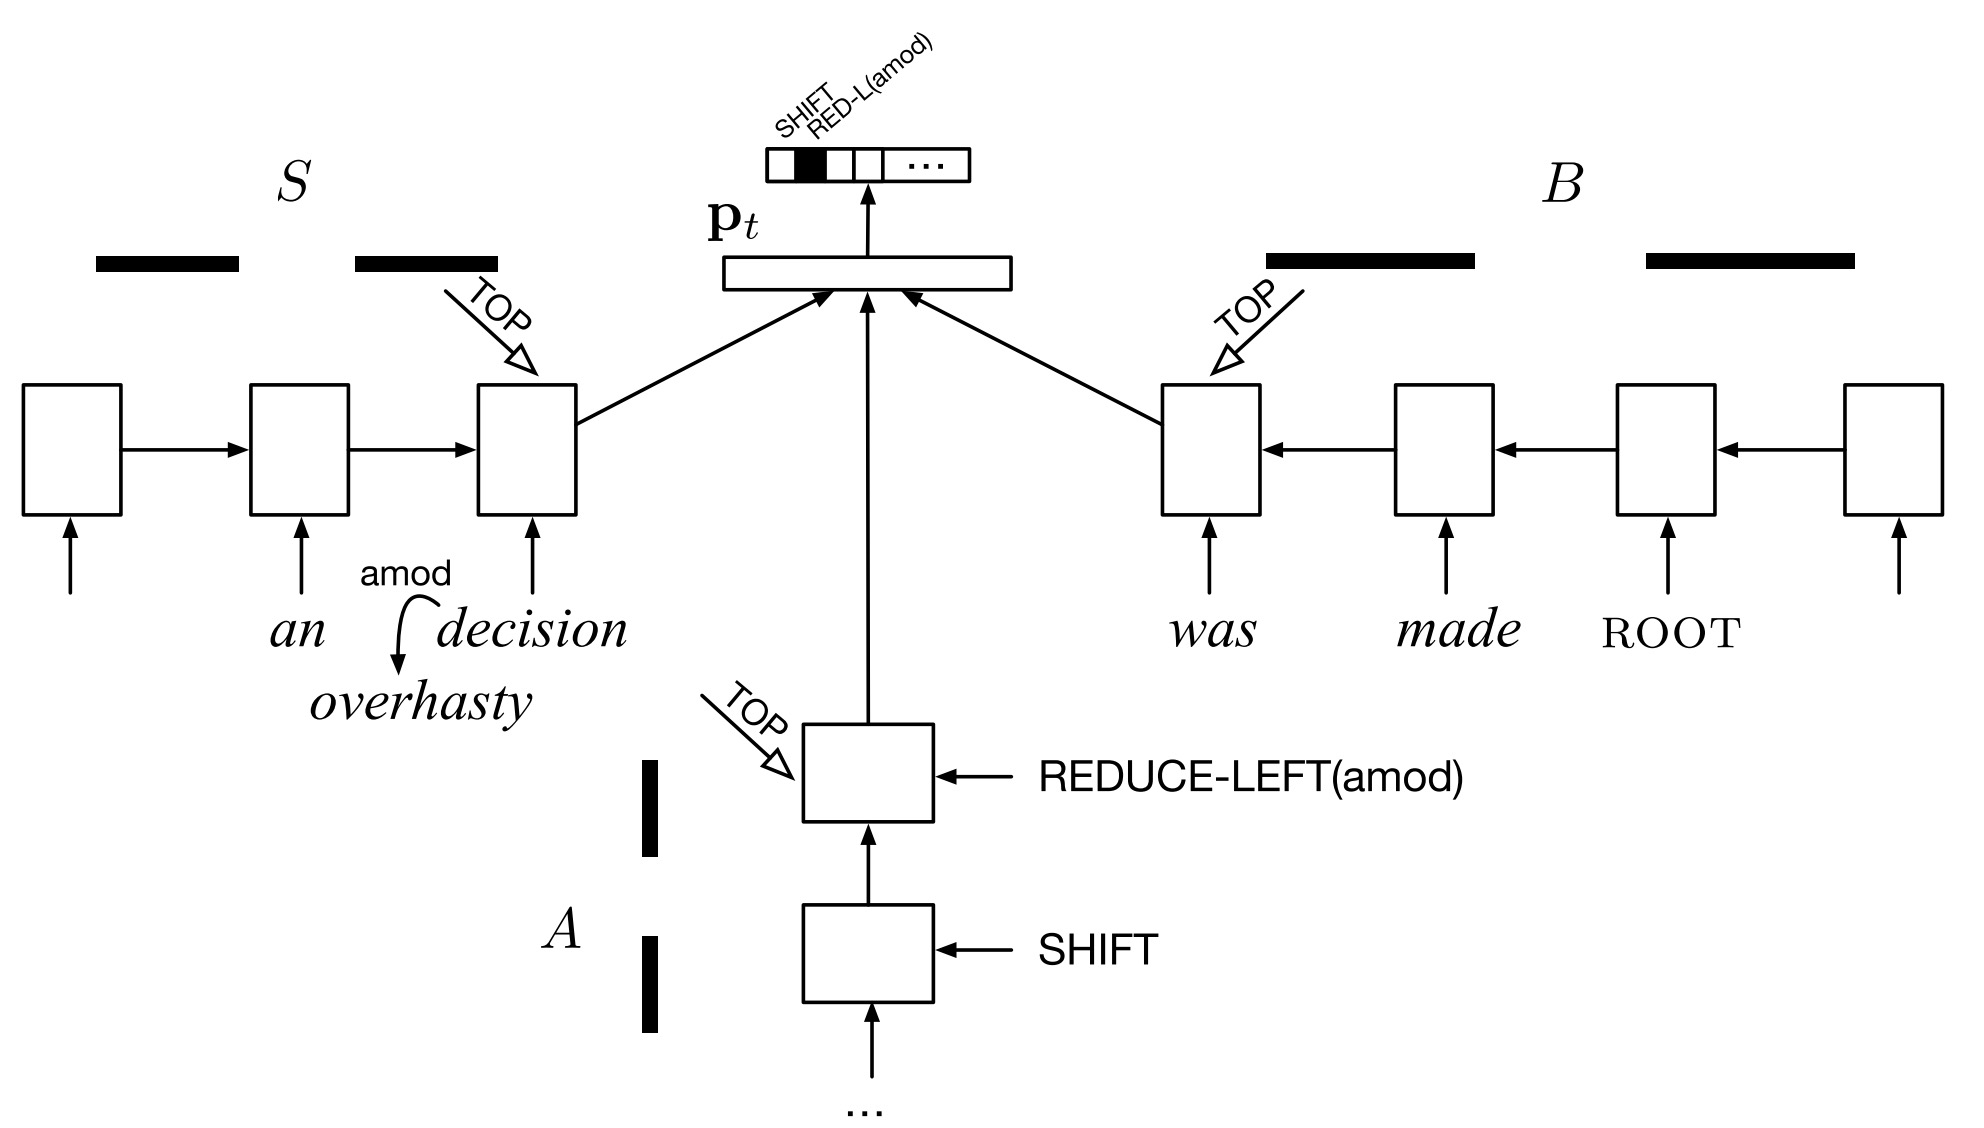
\includegraphics[width=0.8\columnwidth]{distill/dyer}}
	\subfigure{
		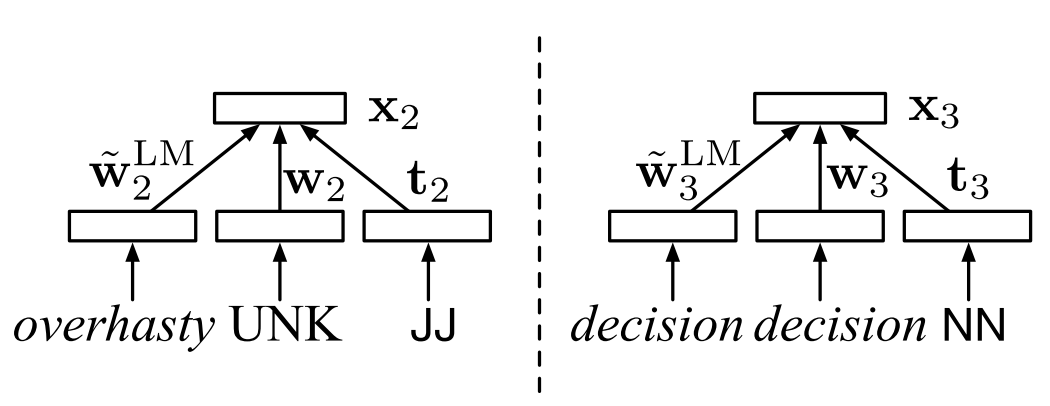
\includegraphics[width=0.5\columnwidth]{distill/inputs}}
	\bicaption{}{文献\inlinecite{dyer-EtAl:2015:ACL-IJCNLP}
		提出的基于转移的依存句法分析器。%左图为PTB实验结果,右图为IWSLT实验结果。
	}{Fig. $\!$}{The parser of Dyer et al. (2015) \inlinecite{dyer-EtAl:2015:ACL-IJCNLP}.
		\label{fig:parser}}
\end{figure}
本章在基于转移的句法分析中验证本章的知识蒸馏方法。
本章的参考文献\inlinecite{dyer-EtAl:2015:ACL-IJCNLP}
提出的stack-lstm parser构建本章的句法分析器。
其框架如图\ref{fig:parser}所示。
对于stack-lstm parser,
其输入词向量包括固定的词向量$\mathbf{p}$
与可调的词向量$\mathbf{w}$,其做法如图\ref{fig:parser}所示。
本章分别尝试对stack-lstm parser的集成模型以及基于上下文相关词向量的模型进行蒸馏。
通过对基于上下文相关词向量的模型进行蒸馏,
本章可以回答本章方法对教师模型与学生模型异构的情况下,
能否通过知识蒸馏的方式达到又快又好的结构预测的效果?

本章在此使用与第\ref{chp:seqlabel}章类似的方式
在基于转移的依存句法分析中加入上下文相关词向量。
即将其各层取平均,作为一种额外的固定的向量表示。
本章待蒸馏的模型则不含有对应的上下文相关词向量。
在这一节,本章使用的蒸馏过程与前文从两种状态中蒸馏的方法相同。

\section{实验}[Experiments]\label{sec:distill:vani-exp}
本章在
%两项任务 --- 基于转移的依存句法分析以及神经机器翻译上
基于转移的依存句法分析进行实验。
本章依据第\ref{sec:distill:sbsp}节
提到的方法将
%两项任务
基于转移的句法分析
转化为基于搜索的结构预测问题。

在基于转移的句法分析的实验中,
本章使用Dyer等人在2015年的文献\inlinecite{dyer-EtAl:2015:ACL-IJCNLP}
中提出的stack-lstm算法建模策略的分类器。\footnote{本章将句法分析代码开源在\url{https://github.com/Oneplus/twpipe}。}
%在神经网络机器翻译的实验中,
%本章使用基于注意力机制的编码器-解码器框架\cite{luong-pham-manning:2015:EMNLP}
%建模策略的分类器。\footnote{本章基于OpenNMT \cite{klein-EtAl:2017:ACL-2017-System-Demonstrations}进行了机器翻译实验并将这部分
%	实验代码开源于\url{https://github.com/Oneplus/OpenNMT-py}。}
%有关模型细节可以参考原文。

\subsection{设置}[Settings]
%\subsubsection{基于转移的依存句法分析}[Transition-based Dependency Parsing]

本章在宾州树库(Penn Treebank,简称PTB,文献\inlinecite{Marcus93buildinga})
数据集上进行实验。
本章使用标准数据划分(2-21节用作训练集,22节用作开发集,23节用作测试集)。
本章参考文献\cite{dyer-EtAl:2015:ACL-IJCNLP}并使用斯坦福依存句法(Stanford dependencies)规范
将短语结构句法转化为依存句法。\footnote{本章使用Stanford CoreNLP 3.3.0 (\url{https://stanfordnlp.github.io/CoreNLP/history.html})完成这一转化。}
本章通过10-折交叉验证获得训练数据的自动词性,其准确率为97.5\%。
本章使用不考虑标点符号的带标签依存关系准确率(LAS)评估通用依赖性分析性能。
本章的模型的超参数参考文献\inlinecite{dyer-EtAl:2015:ACL-IJCNLP}。
最好的迭代轮次由开发集性能决定。

文献\inlinecite{reimers-gurevych:2017:EMNLP2017}
指出神经网络的学习过程是非确定的,所以
汇报单次运行的结果并不能反映模型的性能。
为了消除随机初始化对模型性能的影响,
本章报告了20次随机运行的结果的平均值。

%\subsubsection{神经机器翻译}[Neural Machine Translation]
%\begin{figure}[t]
%	\centering
%	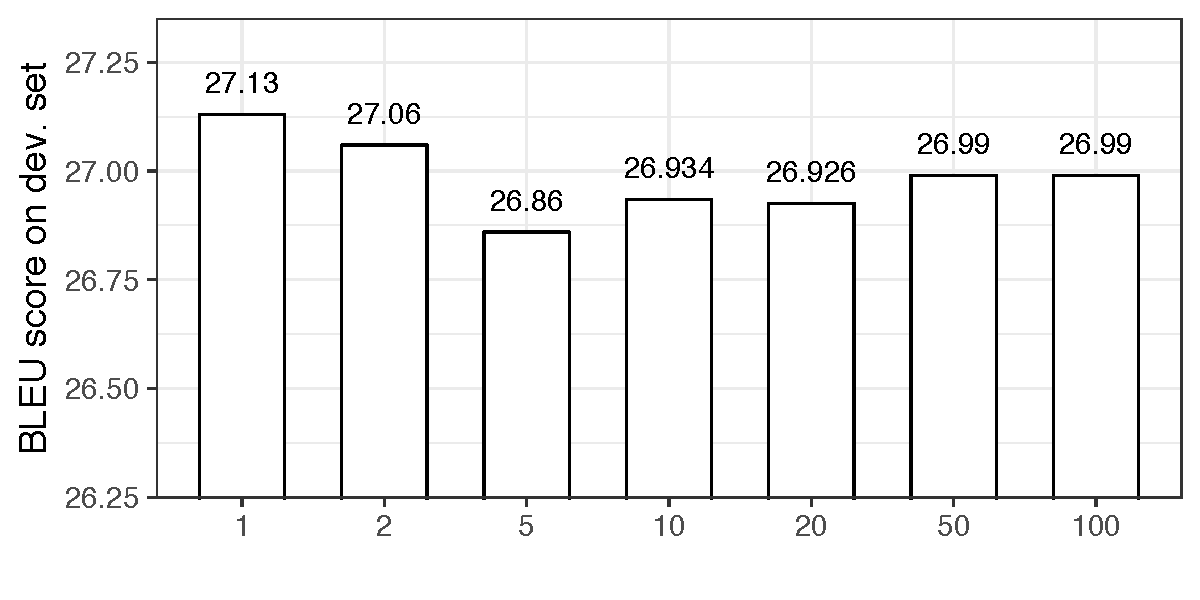
\includegraphics[width=0.7\columnwidth]{distill/approx}
%	\bicaption{}{使用的不同的概率$K$-最大输出对分布进行近似时的机器翻译的效果。}
%	{Fig. $\!$}{The effect of using different $K$s when approximating
%		distillation loss with $K$-most probable actions in the machine translation experiments.\label{fig:distill:approx}}
%\end{figure}
%
%本章在一个IWSLT2014德-英机器翻译数据集上进行实验。
%IWSLT2014德-英机器翻译数据集包含15.3万句训练数据,
%7千句开发集数据,以及7千句测试集数据。
%本章按照文献\inlinecite{DBLP:journals/corr/RanzatoCAZ15}
%建议的方法对数据进行预处理,
%并使用一个包含3万德语词以及2.5万英语词的词表作为模型的词表。
%本章参考文献\inlinecite{wiseman-rush:2016:EMNLP2016}
%并使用含有256个隐层单元的LSTM作为编码器与解码器。
%本章使用BLEU\cite{papineni-EtAl:2002:ACL}评价机器翻译的
%性能。\footnote{本章使用{\tt multi-bleu.perl}脚本评价机器翻译的性能。}
%与依存句法分析实验类似,
%本章汇报10次不同初始化条件下机器翻译模型的平均准确率。
%
%优化公式\ref{eq:distill:distill}需要枚举所有可能的动作。
%在神经机器翻译的情景下,由于词表非常大,
%这种枚举往往是非常耗时耗力的。
%为了使这种枚举可计算,本章使用根据
%集成模型得到的$K$个最可能动作作为
%整个$q(a\mid s)$概率分布的一种近似,
%即优化
%$\sum_a q(a \mid s) \cdot \log p(a \mid s) \approx
%\sum_k^K q(\hat{a}_k \mid s) \cdot \log p(\hat{a}_k \mid s)$学习目标。
%其中$\hat{a}_k$,是第$k$可能的动作。
%为了研究$K$的近似能力,本章将$\alpha$固定为1,
%通过调整$K$观察模型蒸馏的效果。
%图\ref{fig:distill:approx}显示了这一结果。
%从图\ref{fig:distill:approx}可见,$K$的不同并未带来显著的模型差异。
%故出于速度考虑,本章在后续实验中设定$K$为1。

\subsection{结果}[Results]\label{sec:distill:exp-res}

%\subsubsection{基于转移的依存句法分析}[Transition-based Dependency Parsing]
\begin{table}[t]
	\bicaption{}{句法分析的结果。
	显著性检验证明基于知识蒸馏的方法相对基线系统的提升以$p\le 0.01$
	统计显著。}{Table$\!$}{The dependency parsing results. 
		Significance test \cite{NILSSON08.52} shows the improvement of our \textit{Distill (both)} over \textit{Baseline}
		is statistically significant with $p<0.01$.\label{tbl:distill:parse-res}}
	\vspace{0.5em}\centering\wuhao
	\begin{tabular}{lc}
		\toprule[1.5pt]
		& LAS \\
		\midrule[1pt]
		Baseline & 90.83  \\
		Ensemble (20) & 92.73 \\
		Distill (reference, $\alpha$=1.0) & 91.99 \\
		Distill (exploration, $T$=1.0) & 92.00 \\
		Distill (both) & 92.14 \\
		\midrule[0.5pt]
		Ballesteros等人,文献\inlinecite{ballesteros-EtAl:2016:EMNLP2016}  (dyn. oracle) & 91.42 \\
		Andor等人,文献\inlinecite{andor-EtAl:2016:P16-1} (local, B=1) & 91.02 \\
		\midrule[0.5pt]
		Buckman等人,文献\inlinecite{buckman-ballesteros-dyer:2016:EMNLP2016} (local, B=8) & 91.19 \\
		Andor等人,文献\inlinecite{andor-EtAl:2016:P16-1} (local, B=32) & 91.70 \\
		Andor等人,文献\inlinecite{andor-EtAl:2016:P16-1} (global, B=32) & 92.79 \\
		Dozat与Manning,文献\inlinecite{DBLP:journals/corr/DozatM16} & 94.08 \\
		Kuncoro等人,文献\inlinecite{kuncoro-16} & 92.06 \\
		Kuncoro等人,文献\inlinecite{kuncoro-17} & 94.60 \\
		\bottomrule[1.5pt]
	\end{tabular}
\end{table}

\begin{table}[t]
	\bicaption{}{针对基于上下文相关词向量的句法分析的知识蒸馏实验。}
	{Table $\!$}{Distillation from structured prediction model with contextualized embeddings.\label{tbl:elmo-tb-parser}}
	\vspace{0.5em}\centering\wuhao
	\begin{tabular}{lcc}
		\toprule[1.5pt]
		model & LAS & spd. \\
		\midrule[1pt]
		Baseline & 90.83 & 1x \\
		\quad +ELMo & 92.64 & 7.3x \\
%		\quad +ELMo (ensemble 10) & 93.52 & 73x \\
		Distill (both) & 91.80 & 1x \\
		\bottomrule[1.5pt]
	\end{tabular}
\end{table}

表\ref{tbl:distill:parse-res}显示了PTB数据集上的实验结果。
这一结果显示集成模型高于基线模型1.90。
在将$\alpha$设置为1时,模型取得了最佳的开发集结果。
而此时测试集的准确率为91.99。

本章也研究了温度对于从探索状态中蒸馏的模型的影响。
图\ref{fig:distill:temperature}显示了这一结果。
根据表\ref{fig:distill:temperature},
在采样时使用尖锐的分布总体上取得了更好的开发集性能。
从探索状态蒸馏与从参考状态中蒸馏获得的模型的性能基本相当。
将两者结合进一步提高了准确率(带标签的依存关系准确率达到92.14)。

本章也在表\ref{tbl:distill:parse-res}中
将本章提出的模型与其他依存句法分析器进行了对比。
表\ref{tbl:distill:parse-res}的第二组显示了前人工作中
基于贪心解码的依存句法分析器的性能。
文献\inlinecite{andor-EtAl:2016:P16-1}
使用了与本章不同的状态表示方法,
同时分别研究了贪心解码与柱搜索(beam-search)的效果。
文献\inlinecite{ballesteros-EtAl:2016:EMNLP2016}
研究了使用dynamic oracle训练贪心解码的句法分析器
的问题。
本章提出的基于知识蒸馏的句法分析器的表现
好于这些基于贪心解码的句法分析器。
表\ref{tbl:distill:parse-res}显示了
其他依存句法分析算法的效果。
这些算法包括:在基于转移的句法分析中
使用柱搜索\cite{buckman-ballesteros-dyer:2016:EMNLP2016,andor-EtAl:2016:P16-1},
使用全局优化目标训练基于转移的依存句法分析\cite{andor-EtAl:2016:P16-1},
基于图的依存句法分析\cite{DBLP:journals/corr/DozatM16},
将基于图的依存句法分析器蒸馏到基于转移的依存句法分析器\cite{kuncoro-16},
以及将短语结构句法的结果通过规则转化为依存句法\cite{kuncoro-17}。
本章提出的基于知识蒸馏的方法由于这些基于转移的算法,
但相较其他算法仍有差距。
这类差距主要是由对问题的建模方式的不同导致的。

除了对集成模型进行蒸馏,
本章也尝试对基于上下文相关词向量的句法分析器进行蒸馏。
其实验结果如表\ref{tbl:elmo-tb-parser}所示。
根据表\ref{tbl:elmo-tb-parser},
使用本章提出的知识蒸馏方法可以从异构模型中有效地学习模型。
从而使用简单模型达到与使用上下文相关词向量模型类似的性能。
由于本章简单模型不使用上下文相关词向量,
所以,这一方法显著优化了模型速度。

%
%\subsubsection{神经机器翻译}[Neural Machine Translation]
%
%\begin{table}[t]
%	\bicaption{}{神经机器翻译的结果。
%		MIX代表文献\inlinecite{DBLP:journals/corr/RanzatoCAZ15}提出的基于强化学习的算法。
%		BSO代表文献\inlinecite{wiseman-rush:2016:EMNLP2016}提出的基于全局学习的算法。
%		显著性检验\cite{koehn:2004:EMNLP}证明基于知识蒸馏的方法相对基线系统的提升以$p\le 0.01$
%		统计显著。
%	}{Table$\!$}{The machine translation results.
%		MIXER denotes that of \inlinecite{DBLP:journals/corr/RanzatoCAZ15},
%		BSO  denotes that of \inlinecite{wiseman-rush:2016:EMNLP2016}.
%		Significance test \cite{koehn:2004:EMNLP} shows the improvement of our \textit{Distill (both)} over \textit{Baseline}
%		is statistically significant with $p<0.01$.\label{tbl:distill:nmt-res}}
%	\vspace{0.5em}\centering\wuhao
%	\begin{tabular}{lc}
%		\toprule[1.5pt]
%		& BLEU \\
%		\midrule[1pt]
%		Baseline & 22.79 \\
%		Ensemble (10) & 26.26 \\
%		Distill (reference, $\alpha$=0.8) & 24.76 \\
%		Distill (exploration, $T$=0.1) & 24.64 \\
%		Distill (both) & 25.44 \\
%		\midrule[0.5pt]
%		MIXER & 20.73 \\
%		BSO (local, B=1) & 22.53 \\
%		BSO (global, B=1) & 23.83 \\
%		\bottomrule[1.5pt]
%	\end{tabular}
%\end{table}
%
\begin{figure}[t]
	\centering
	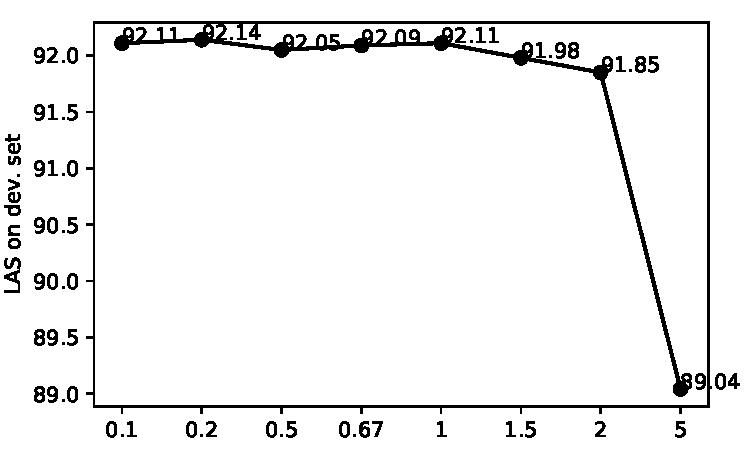
\includegraphics[width=0.6\textwidth]{distill/temperature}
	\bicaption{}{温度参数$T$对模型性能的影响。
		%左图显示的是句法分析的结果,右图显示的机器翻译的结果。
	}{Fig. $\!$}{The effect of $T$ on %PTB (left)
		%and IWSLT 2014 (right) 
		development set.\label{fig:distill:temperature}
	}
\end{figure}
%
%表\ref{tbl:distill:nmt-res}显示了IWSLT 2014数据集的机器翻译结果。
%与PTB的结果类似的是,对10个模型进行集成的效果超过
%基线系统3.47个BLEU值。
%从参考状态中进行知识蒸馏能够获得BLEU值为24.76的单模型。
%
%与基于转移的句法分析实验类似的是,
%在采样过程中尖锐的分布带来的模型的效果更好,
%然而,根据图\ref{fig:distill:temperature},
%在$T\le0.2$的情况下,$T$的不同导致的差异并不明显。
%在后续实验中,本章根据开发集结果设定$T=0.1$。
%表\ref{tbl:distill:nmt-res}显示从探索状态中进行知识蒸馏的
%模型获得24.64的准确率。
%这一准确率相机从参考状态中蒸馏有微小的差异。
%但将从参考中蒸馏和从探索中蒸馏进一步大幅度提高了准确率,
%并且获得了25.44的BLEU值。
%
%本章也将本章的模型与前人工作进行对比:
%对比的系统包括基于强化学习的机器翻译\cite{DBLP:journals/corr/RanzatoCAZ15},
%以及在翻译器学习过程中加入柱搜索\cite{wiseman-rush:2016:EMNLP2016}。
%对比显示本章提出的模型取得了最优的结果。
%
%上述句法分析与机器翻译实验
%表明仅从探索状态中进行知识蒸馏是可行的。
%同时将从参考状态中蒸馏与从探索状态中蒸馏进行结合可以进一步提高模型
%性能,并取得超越其他贪心搜索模型的性能。

%\paragraph{Speed Comparison}
%
%\begin{table}
%	\centering
%	\begin{tabular}{rrcc}
%		\hline
%		model & beam & BLEU & speed \\
%		Baseline & 1 & & \\
%		& 5 & & \\
%		& 10 & & \\
%		\hline
%		Distill both & & & \\
%		\hline
%	\end{tabular}
%\caption{Speed comparison.}
%\end{table}
%
%Beam search generally improves search-based structured predictor's perform
%according to previous literals \cite{buckman-ballesteros-dyer:2016:EMNLP2016,wiseman-rush:2016:EMNLP2016}.
%We run a beam-search decoding on the baseline model.

\subsection{分析}[Analysis]\label{sec:analysis}

根据第\ref{sec:distill:exp-res}节的结果,
使用集成模型显著提高了依存句法分析以及神经机器翻译的性能够。
然而,类似``为什么集成模型如此有效?
能不能放弃传统对数似然学习目标,完全从知识蒸馏学习目标中学习?
以及从知识蒸馏中学习是不是稳定的?''一类的问题并没有得到很好的回答。
在这一节中,
本章首先研究集成模型在``错误状态''上的表现
证明其具有更好的泛化能力。
然后,本章通过研究公式\ref{eq:distill:distill}中的$a$的作用
经验性地证明了完全从知识蒸馏中学习的可行性。
最后,本章通过分析表明知识蒸馏可以带来更稳定的模型学习。

\subsubsection{模型集成对于``错误状态''的作用}[Ensemble on ``Problematic'' States]\label{sec:distill:ens-on-states}
\begin{table}[t]
	\bicaption{}{不同模型的``错误状态''的排序性能。}{Table $\!$}{The ranking performance of parsers' 
		output distributions evaluated in MAP on
		``problematic'' states.\label{tbl:state-ana}}
	\vspace{0.5em}\centering\wuhao
	\begin{tabular}{l  c c}
		\toprule[1.5pt]
		& 有歧义的正确状态 & 非正确状态 \\
		\midrule[1pt]
		Baseline & 68.59 & 89.59\\
		Ensemble & 74.19 & 90.90 \\
		Distill (both) & 81.15 & 91.38 \\
		\bottomrule[1.5pt]
	\end{tabular}
\end{table}
如前文所述,歧义或者非最优的``错误状态''影响结构预测的准确率。
根据第\ref{sec:distill:exp-res}节的结果,模型集成能够提升性能,
这表明其能够更好地处理``错误状态''。
为了经验性地验证这一假设,
本章以依存句法分析为目标,
借助dynamic oracle研究集成模型的输出分布。

dynamic oracle\cite{goldberg-nivre:2012:PAPERS,TACL302} 
能够有效地判断,对于一棵句法树的任意给定状态$s$,
最优的转移动作(\textit{参考动作})是什么。
这里``最优''指的是能够搜索得到的相似度(用LAS衡量)最高的树。
这种性质使得本章可以对``错误状态''中的某个动作进行分析。
本章根据\textit{参考动作}
评价了基线模型以及集成模型在动作空间上输出的分布。
由于dynamic oracle会对一个状态给出多个参考动作,
本章将这一评价问题转化为一个排序的评价问题。
直观来讲,当多个参考动作存在是,
一个好的句法分析器应当将动作的概率密度集中在参考动作上。
本章通过随机采样从基线模型中获得了一系列状态。
不同模型的排序分数如表\ref{tbl:state-ana}所示。
根据表\ref{tbl:state-ana},
集成模型在``错误状态''下的排序表现更好。
这一观察表明,集成模型的输出分布所包含的信息更丰富,
因而在``错误状态''上表现得更好,并取得更好的性能。
同时,本章也观察到蒸馏模型的性能好于基线与集成模型。
本章认为造成这一现象的原因是蒸馏模型的学习过程包含探索机制。

\subsubsection{$\alpha$的效果}[Effect of $\alpha$]
\begin{figure}[t]
	\centering
	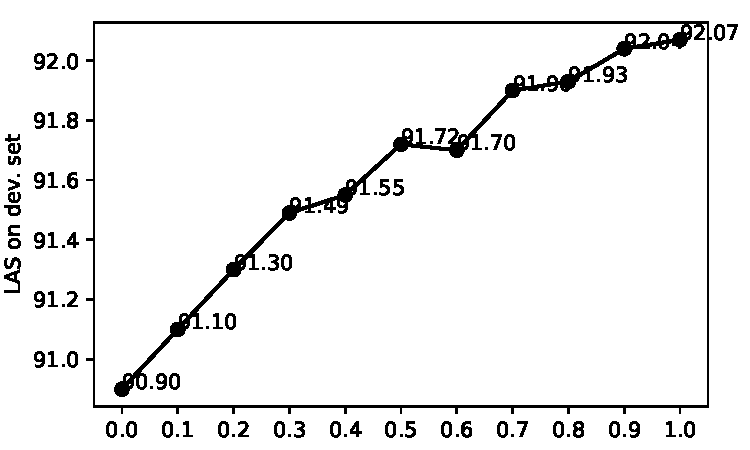
\includegraphics[width=0.6\columnwidth]{distill/alpha}
	\bicaption{}{开发集上$\alpha$值的效果%左图为PTB实验结果,右图为IWSLT实验结果。
	}{Fig. $\!$}{The effect of $\alpha$% on PTB (left)
		%and IWSLT 2014 (right) development set.
		\label{fig:alpha}}
\end{figure}

本章在从参考状态中蒸馏模型的学习过程中研究$\alpha$的影响。
本章在基于转移的句法分析以及神经机器翻译中将$\alpha$从0到1以0.1为步长变化,
并在图\ref{fig:alpha}中展示了模型的性能。
两个实验都显示大$\alpha$的表现好于小$\alpha$。
对于句法分析,$\alpha=1$时取得了最好的开发集性能。
对于神经机器翻译,开发集性能最好的$\alpha$是0.8。
同时,在机器翻译实验中,$\alpha=0.8$与$\alpha=1$的模型只有0.2的差距。
这一系列观察表明对于从参考状态时,
更多地关注知识蒸馏的学习目标能够带来更好的模型性。
这一观察也显示对于从探索状态中蒸馏模型(即$\alpha=1$)
的可行性。

\subsubsection{模型学习的稳定性}[Learning Stability]
\begin{figure}[t]
	\centering
	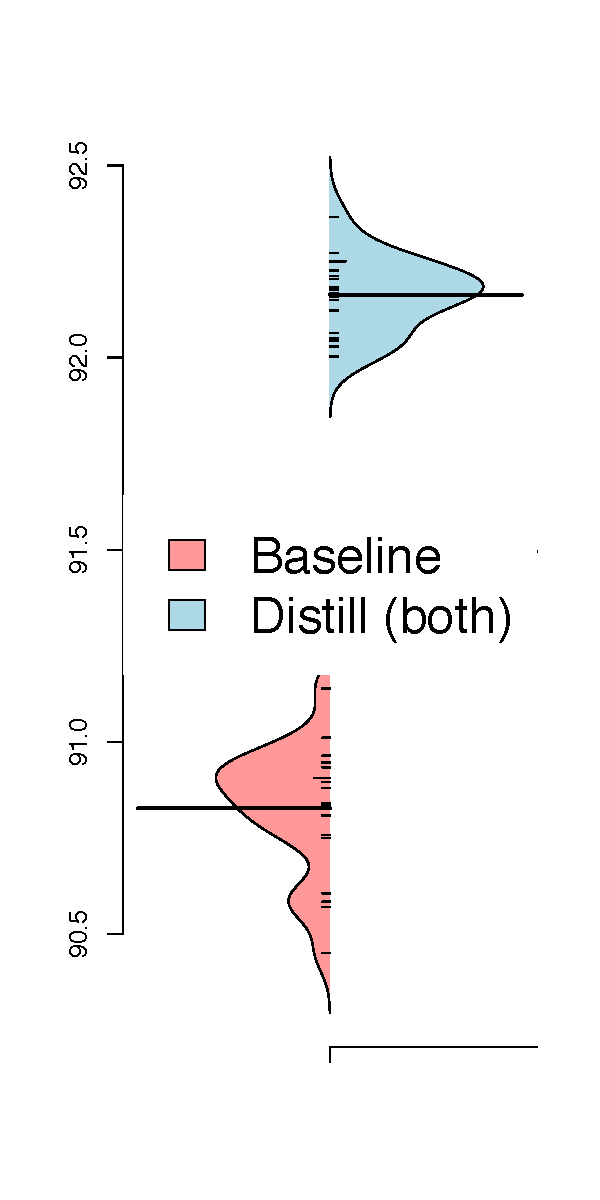
\includegraphics[width=0.3\columnwidth, trim={0, 1cm, 0, 1.5cm}, clip]{distill/stability_par_bean}
%	\subfigure{\includegraphics[width=0.3\columnwidth, trim={0, 1cm, 0, 1.5cm}, clip]{distill/stability_nmt_bean}}
	\bicaption{}{不同随机种子下模型分数的分布。
		%左图显示PTB上测试集的结果,右图显示IWSLT上测试集的结果。
	}{Fig. $\!$}{The distributions of scores for the baseline model and
		our {\it distillation from both} on PTB
		% test (left) and IWSLT 2014 test (right)
		on differently-seeded runs.\label{fig:stable}}
\end{figure}

\begin{table}[t]
	\bicaption{}{结果的最大值、最小值以及标准差。}{Table $\!$}{The minimal, maximum, and standard derivation values
		on differently-seeded runs.\label{tbl:stable}}
	\vspace{0.5em}\centering\wuhao
	\begin{tabular}{rcccc}
		\toprule[1.5pt]
		system & seeds & min & max & $\sigma$ \\
		\midrule[1pt]
		\multicolumn{2}{r}{\it PTB test} & & & \\
		Baseline & 20 & 90.45 & 91.14 & 0.17 \\
		Distill (both) & 20 & 92.00 & 92.37 & 0.09 \\
%		\midrule[0.5pt]
%		\midrule[0.5pt]
%		\multicolumn{2}{r}{\it IWSLT 2014 test} & & & \\
%		Baseline & 10 & 21.63 & 23.67 & 0.55 \\
%		Distill (both) & 10 & 24.22 & 25.65 & 0.12 \\
		\bottomrule[1.5pt]
	\end{tabular}
\end{table}
除了提高性能,
知识蒸馏也能给模型学习的稳定性带来提升。
本章将不同随机种子得到的基线模型与蒸馏模型的准确率
以琴图的方式绘制在图\ref{fig:stable}中,
同时在表\ref{tbl:stable}中显示了两种模型的标准差。
可见,知识蒸馏模型的标准差更小,
即其学习更稳定。
文献\inlinecite{DBLP:journals/corr/KeskarMNST16}指出
影响神经网络模型的泛化性能的主要问题并非过拟合,
而是模型参数进入尖锐的局部极小点(sharp minimizer)。
这种局部极小点的泛化性往往较差。
根据这一理论,本章猜测知识蒸馏取得更稳定的训练效果的原因是
知识蒸馏的学习曲目更光滑,尖锐的局部极小点更少。

\section{相关工作}[Related Work]

前人工作中有若干在NLP任务中使用知识蒸馏技术。
Kim与Rush在2016年的文献\inlinecite{kim-rush:2016:EMNLP2016}
中关注如将复杂模型蒸馏到简单模型中。
同时,他们的方法主要关注序列级别的蒸馏。
与之相反的是,本章更关注动作级的知识蒸馏,
同时提出从参考状态以及从探索状态中进行知识蒸馏。

Freitag等人在2017年的文献\inlinecite{DBLP:journals/corr/FreitagAS17}
中使用六个翻译器的译文生成翻译的训练数据,
其模型使用柱搜索进行探索。
与其不同的是,
本章使用单模型产生训练数据,并以拟合集成模型的分布为学习目标。

在强化学习中,
集成模型的探索机制也得到了相应的研究\cite{NIPS2016_6501}。
除了在标注数据上蒸馏模型,
也有一部分半监督学习的工作从生语料上进行模型学习\cite{liang:icml08,li-zhang-chen:2014:P14-1}。
如何在生语料上进行知识蒸馏也值得后续工作的研究。

Kuncoro在2016年的文献\inlinecite{kuncoro-16}
中提出将20个基于转移的句法分析器的结果通过投票的方式进行集成并
将结果以后验正则的方式应用于训练一个基于图的模型。
不同于他们的模型,将基于转移的模型蒸馏到基于转移的模型中。

除了使用知识蒸馏,
Stahlberg等人在2017年的文献\inlinecite{stahlberg-byrne:2017:EMNLP2017}
中提出将若干翻译模型的集成组合为一个神经网络,并用SVD化简了模型。
他们的模型也可以视作一种知识蒸馏。

\section{本章小结}[Conclusion]
本章研究了结构预测中的知识蒸馏问题。
本章提出将若干模型的模型集成蒸馏到一个单模型中。
这一蒸馏过程同时在参考状态以及探索状态中完成。
在基于转移的句法分析
%以及神经机器翻译
实验中,
本章模型获得了显著的性能提升,从而证明了本章提出的方法的有效性。
同时,本章通过分析给出了本章知识蒸馏方法可行性的验证。

在此基础上,
本章对于基于上下文相关词向量的句法分析器进行知识蒸馏。
实验结果显示本章提出的方法对于异构模型同样有效,
在少量损失精度的情况下近十倍地提高模型速度。